\documentclass[twoside]{book}

% Packages required by doxygen
\usepackage{calc}
\usepackage{doxygen}
\usepackage{graphicx}
\usepackage[utf8]{inputenc}
\usepackage{makeidx}
\usepackage{multicol}
\usepackage{multirow}
\usepackage{textcomp}
\usepackage[table]{xcolor}

% Font selection
\usepackage[T1]{fontenc}
\usepackage{mathptmx}
\usepackage[scaled=.90]{helvet}
\usepackage{courier}
\usepackage{amssymb}
\usepackage{sectsty}
\renewcommand{\familydefault}{\sfdefault}
\allsectionsfont{%
  \fontseries{bc}\selectfont%
  \color{darkgray}%
}
\renewcommand{\DoxyLabelFont}{%
  \fontseries{bc}\selectfont%
  \color{darkgray}%
}

% Page & text layout
\usepackage{geometry}
\geometry{%
  a4paper,%
  top=2.5cm,%
  bottom=2.5cm,%
  left=2.5cm,%
  right=2.5cm%
}
\tolerance=750
\hfuzz=15pt
\hbadness=750
\setlength{\emergencystretch}{15pt}
\setlength{\parindent}{0cm}
\setlength{\parskip}{0.2cm}
\makeatletter
\renewcommand{\paragraph}{%
  \@startsection{paragraph}{4}{0ex}{-1.0ex}{1.0ex}{%
    \normalfont\normalsize\bfseries\SS@parafont%
  }%
}
\renewcommand{\subparagraph}{%
  \@startsection{subparagraph}{5}{0ex}{-1.0ex}{1.0ex}{%
    \normalfont\normalsize\bfseries\SS@subparafont%
  }%
}
\makeatother

% Headers & footers
\usepackage{fancyhdr}
\pagestyle{fancyplain}
\fancyhead[LE]{\fancyplain{}{\bfseries\thepage}}
\fancyhead[CE]{\fancyplain{}{}}
\fancyhead[RE]{\fancyplain{}{\bfseries\leftmark}}
\fancyhead[LO]{\fancyplain{}{\bfseries\rightmark}}
\fancyhead[CO]{\fancyplain{}{}}
\fancyhead[RO]{\fancyplain{}{\bfseries\thepage}}
\fancyfoot[LE]{\fancyplain{}{}}
\fancyfoot[CE]{\fancyplain{}{}}
\fancyfoot[RE]{\fancyplain{}{\bfseries\scriptsize Generated on Wed Jul 2 2014 12\-:21\-:46 for My Project by Doxygen }}
\fancyfoot[LO]{\fancyplain{}{\bfseries\scriptsize Generated on Wed Jul 2 2014 12\-:21\-:46 for My Project by Doxygen }}
\fancyfoot[CO]{\fancyplain{}{}}
\fancyfoot[RO]{\fancyplain{}{}}
\renewcommand{\footrulewidth}{0.4pt}
\renewcommand{\chaptermark}[1]{%
  \markboth{#1}{}%
}
\renewcommand{\sectionmark}[1]{%
  \markright{\thesection\ #1}%
}

% Indices & bibliography
\usepackage{natbib}
\usepackage[titles]{tocloft}
\setcounter{tocdepth}{3}
\setcounter{secnumdepth}{5}
\makeindex

% Hyperlinks (required, but should be loaded last)
\usepackage{ifpdf}
\ifpdf
  \usepackage[pdftex,pagebackref=true]{hyperref}
\else
  \usepackage[ps2pdf,pagebackref=true]{hyperref}
\fi
\hypersetup{%
  colorlinks=true,%
  linkcolor=blue,%
  citecolor=blue,%
  unicode%
}

% Custom commands
\newcommand{\clearemptydoublepage}{%
  \newpage{\pagestyle{empty}\cleardoublepage}%
}


%===== C O N T E N T S =====

\begin{document}

% Titlepage & ToC
\hypersetup{pageanchor=false}
\pagenumbering{roman}
\begin{titlepage}
\vspace*{7cm}
\begin{center}%
{\Large My Project }\\
\vspace*{1cm}
{\large Generated by Doxygen 1.8.6}\\
\vspace*{0.5cm}
{\small Wed Jul 2 2014 12:21:46}\\
\end{center}
\end{titlepage}
\clearemptydoublepage
\tableofcontents
\clearemptydoublepage
\pagenumbering{arabic}
\hypersetup{pageanchor=true}

%--- Begin generated contents ---
\chapter{Hierarchical Index}
\section{Hierarquia de classes}
Esta lista de heranças está organizada, dentro do possível, por ordem alfabética\-:\begin{DoxyCompactList}
\item Q\-Abstract\-Item\-Model\begin{DoxyCompactList}
\item \contentsline{section}{Playlist\-Model}{\pageref{class_playlist_model}}{}
\end{DoxyCompactList}
\item Q\-Main\-Window\begin{DoxyCompactList}
\item \contentsline{section}{Main\-Window}{\pageref{class_main_window}}{}
\end{DoxyCompactList}
\item Q\-Object\begin{DoxyCompactList}
\item \contentsline{section}{Buffer\-Processor}{\pageref{class_buffer_processor}}{}
\item \contentsline{section}{F\-F\-T\-Calc}{\pageref{class_f_f_t_calc}}{}
\end{DoxyCompactList}
\item Q\-Widget\begin{DoxyCompactList}
\item \contentsline{section}{Abstract\-Control}{\pageref{class_abstract_control}}{}
\begin{DoxyCompactList}
\item \contentsline{section}{Controls}{\pageref{class_controls}}{}
\end{DoxyCompactList}
\item \contentsline{section}{Abstract\-Media\-Info}{\pageref{class_abstract_media_info}}{}
\begin{DoxyCompactList}
\item \contentsline{section}{Media\-Info}{\pageref{class_media_info}}{}
\end{DoxyCompactList}
\item \contentsline{section}{Abstract\-Spectrograph}{\pageref{class_abstract_spectrograph}}{}
\begin{DoxyCompactList}
\item \contentsline{section}{Spectrograph}{\pageref{class_spectrograph}}{}
\end{DoxyCompactList}
\end{DoxyCompactList}
\end{DoxyCompactList}

\chapter{Class Index}
\section{Lista de componentes}
Lista de classes, estruturas, uniões e interfaces com uma breve descrição\-:\begin{DoxyCompactList}
\item\contentsline{section}{\hyperlink{class_abstract_control}{Abstract\-Control} }{\pageref{class_abstract_control}}{}
\item\contentsline{section}{\hyperlink{class_abstract_media_info}{Abstract\-Media\-Info} }{\pageref{class_abstract_media_info}}{}
\item\contentsline{section}{\hyperlink{class_abstract_spectrograph}{Abstract\-Spectrograph} }{\pageref{class_abstract_spectrograph}}{}
\item\contentsline{section}{\hyperlink{class_buffer_processor}{Buffer\-Processor} }{\pageref{class_buffer_processor}}{}
\item\contentsline{section}{\hyperlink{class_controls}{Controls} }{\pageref{class_controls}}{}
\item\contentsline{section}{\hyperlink{class_f_f_t_calc}{F\-F\-T\-Calc} }{\pageref{class_f_f_t_calc}}{}
\item\contentsline{section}{\hyperlink{class_main_window}{Main\-Window} }{\pageref{class_main_window}}{}
\item\contentsline{section}{\hyperlink{class_media_info}{Media\-Info} }{\pageref{class_media_info}}{}
\item\contentsline{section}{\hyperlink{class_playlist_model}{Playlist\-Model} }{\pageref{class_playlist_model}}{}
\item\contentsline{section}{\hyperlink{class_spectrograph}{Spectrograph} }{\pageref{class_spectrograph}}{}
\end{DoxyCompactList}

\chapter{Class Documentation}
\hypertarget{class_abstract_control}{\section{Abstract\-Control Class Reference}
\label{class_abstract_control}\index{Abstract\-Control@{Abstract\-Control}}
}


{\ttfamily \#include $<$abstractcontrol.\-h$>$}

Inheritance diagram for Abstract\-Control\-:\begin{figure}[H]
\begin{center}
\leavevmode
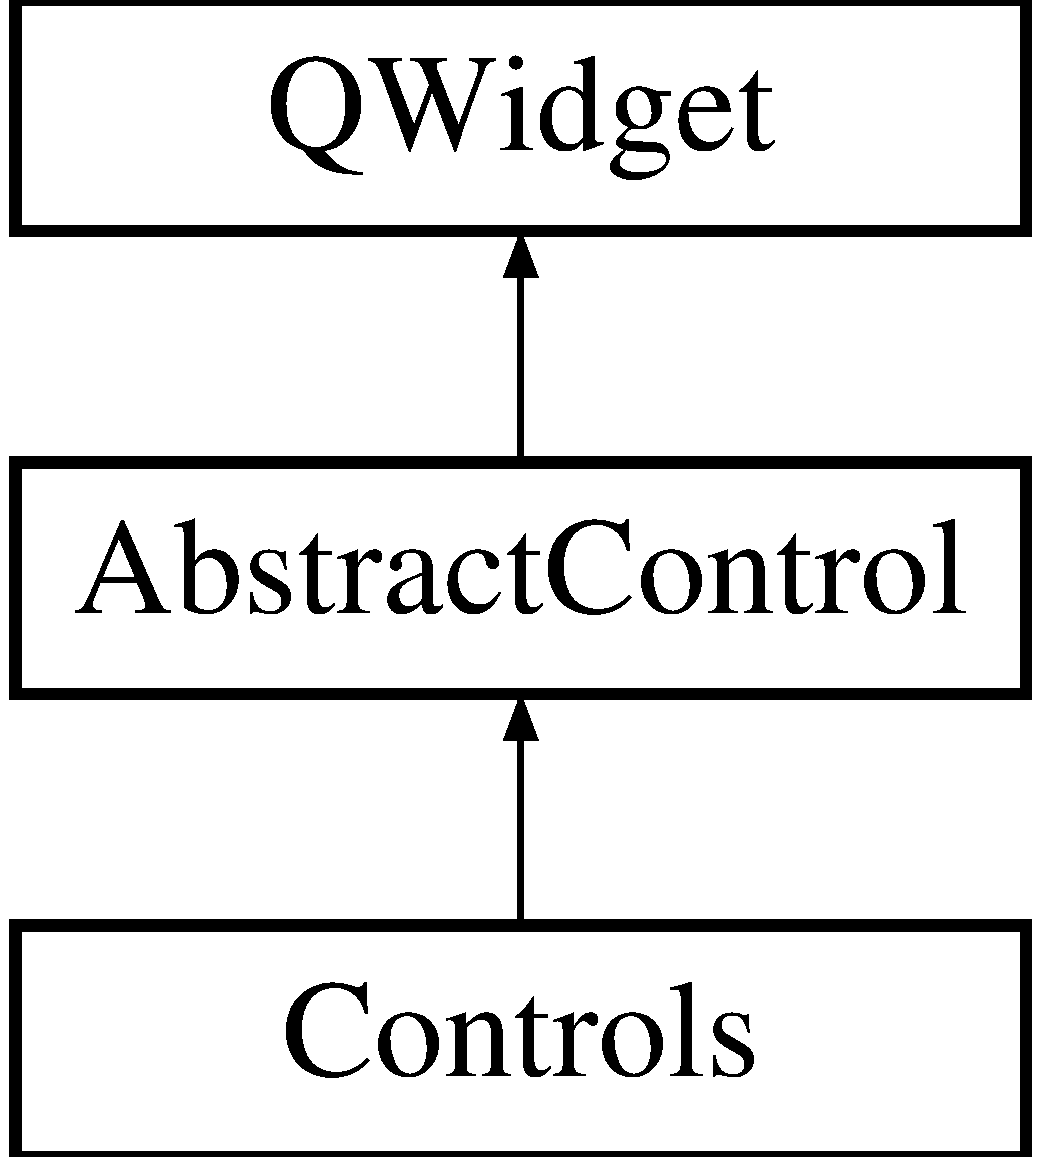
\includegraphics[height=3.000000cm]{class_abstract_control}
\end{center}
\end{figure}
\subsection*{Public Slots}
\begin{DoxyCompactItemize}
\item 
virtual void \hyperlink{class_abstract_control_a99d0d68402b7546c624e6bb7696ee95d}{on\-Play\-Pause\-Clicked} (void)=0
\item 
virtual void \hyperlink{class_abstract_control_abdb7309086319e82a30dfbccea290d60}{on\-Prev\-Clicked} (void)=0
\item 
virtual void \hyperlink{class_abstract_control_a45d6fe6a83a66ae6f69e3b631fbdd547}{on\-Next\-Clicked} (void)=0
\item 
virtual void \hyperlink{class_abstract_control_a0d76bc546bc9bb2be13573814f43ede2}{on\-Volume\-Changed} (int)=0
\item 
virtual void \hyperlink{class_abstract_control_a4aa7cd659eddd599b03df5d905cc1806}{on\-Elapsed\-Changed} (qint64)=0
\item 
virtual void \hyperlink{class_abstract_control_a536755040aecaba6aff81a1704801ef6}{on\-Duration\-Changed} (qint64)=0
\end{DoxyCompactItemize}
\subsection*{Signals}
\begin{DoxyCompactItemize}
\item 
void \hyperlink{class_abstract_control_ad2e9ced2f1cc8843b0d41aed65147940}{play\-Pause} ()
\item 
void \hyperlink{class_abstract_control_a2d22cb619310c6e5124714f50752785e}{next} ()
\item 
void \hyperlink{class_abstract_control_a4d4c1291abf6badfcc50bc5b0f29a4e7}{prev} ()
\item 
void \hyperlink{class_abstract_control_a8deefe7ec20ba2828132c0f4dd7ec2d2}{stop} ()
\item 
void \hyperlink{class_abstract_control_ab87486a10333c41af89e9f2f1e4aa00b}{volume\-Selected} (int)
\item 
void \hyperlink{class_abstract_control_a4ef5f5771ae42561aec365a9aabe4615}{elapsed\-Selected} (qint64)
\end{DoxyCompactItemize}
\subsection*{Public Member Functions}
\begin{DoxyCompactItemize}
\item 
\hyperlink{class_abstract_control_a2caef38ad55c0589a073a3ead352c7ad}{Abstract\-Control} (Q\-Widget $\ast$parent=0)
\end{DoxyCompactItemize}


\subsection{Constructor \& Destructor Documentation}
\hypertarget{class_abstract_control_a2caef38ad55c0589a073a3ead352c7ad}{\index{Abstract\-Control@{Abstract\-Control}!Abstract\-Control@{Abstract\-Control}}
\index{Abstract\-Control@{Abstract\-Control}!AbstractControl@{Abstract\-Control}}
\subsubsection[{Abstract\-Control}]{\setlength{\rightskip}{0pt plus 5cm}Abstract\-Control\-::\-Abstract\-Control (
\begin{DoxyParamCaption}
\item[{Q\-Widget $\ast$}]{parent = {\ttfamily 0}}
\end{DoxyParamCaption}
)\hspace{0.3cm}{\ttfamily [inline]}, {\ttfamily [explicit]}}}\label{class_abstract_control_a2caef38ad55c0589a073a3ead352c7ad}


\subsection{Member Function Documentation}
\hypertarget{class_abstract_control_a4ef5f5771ae42561aec365a9aabe4615}{\index{Abstract\-Control@{Abstract\-Control}!elapsed\-Selected@{elapsed\-Selected}}
\index{elapsed\-Selected@{elapsed\-Selected}!AbstractControl@{Abstract\-Control}}
\subsubsection[{elapsed\-Selected}]{\setlength{\rightskip}{0pt plus 5cm}void Abstract\-Control\-::elapsed\-Selected (
\begin{DoxyParamCaption}
\item[{qint64}]{}
\end{DoxyParamCaption}
)\hspace{0.3cm}{\ttfamily [signal]}}}\label{class_abstract_control_a4ef5f5771ae42561aec365a9aabe4615}
\hypertarget{class_abstract_control_a2d22cb619310c6e5124714f50752785e}{\index{Abstract\-Control@{Abstract\-Control}!next@{next}}
\index{next@{next}!AbstractControl@{Abstract\-Control}}
\subsubsection[{next}]{\setlength{\rightskip}{0pt plus 5cm}void Abstract\-Control\-::next (
\begin{DoxyParamCaption}
{}
\end{DoxyParamCaption}
)\hspace{0.3cm}{\ttfamily [signal]}}}\label{class_abstract_control_a2d22cb619310c6e5124714f50752785e}
\hypertarget{class_abstract_control_a536755040aecaba6aff81a1704801ef6}{\index{Abstract\-Control@{Abstract\-Control}!on\-Duration\-Changed@{on\-Duration\-Changed}}
\index{on\-Duration\-Changed@{on\-Duration\-Changed}!AbstractControl@{Abstract\-Control}}
\subsubsection[{on\-Duration\-Changed}]{\setlength{\rightskip}{0pt plus 5cm}virtual void Abstract\-Control\-::on\-Duration\-Changed (
\begin{DoxyParamCaption}
\item[{qint64}]{}
\end{DoxyParamCaption}
)\hspace{0.3cm}{\ttfamily [pure virtual]}, {\ttfamily [slot]}}}\label{class_abstract_control_a536755040aecaba6aff81a1704801ef6}
\hypertarget{class_abstract_control_a4aa7cd659eddd599b03df5d905cc1806}{\index{Abstract\-Control@{Abstract\-Control}!on\-Elapsed\-Changed@{on\-Elapsed\-Changed}}
\index{on\-Elapsed\-Changed@{on\-Elapsed\-Changed}!AbstractControl@{Abstract\-Control}}
\subsubsection[{on\-Elapsed\-Changed}]{\setlength{\rightskip}{0pt plus 5cm}virtual void Abstract\-Control\-::on\-Elapsed\-Changed (
\begin{DoxyParamCaption}
\item[{qint64}]{}
\end{DoxyParamCaption}
)\hspace{0.3cm}{\ttfamily [pure virtual]}, {\ttfamily [slot]}}}\label{class_abstract_control_a4aa7cd659eddd599b03df5d905cc1806}
\hypertarget{class_abstract_control_a45d6fe6a83a66ae6f69e3b631fbdd547}{\index{Abstract\-Control@{Abstract\-Control}!on\-Next\-Clicked@{on\-Next\-Clicked}}
\index{on\-Next\-Clicked@{on\-Next\-Clicked}!AbstractControl@{Abstract\-Control}}
\subsubsection[{on\-Next\-Clicked}]{\setlength{\rightskip}{0pt plus 5cm}virtual void Abstract\-Control\-::on\-Next\-Clicked (
\begin{DoxyParamCaption}
\item[{void}]{}
\end{DoxyParamCaption}
)\hspace{0.3cm}{\ttfamily [pure virtual]}, {\ttfamily [slot]}}}\label{class_abstract_control_a45d6fe6a83a66ae6f69e3b631fbdd547}
\hypertarget{class_abstract_control_a99d0d68402b7546c624e6bb7696ee95d}{\index{Abstract\-Control@{Abstract\-Control}!on\-Play\-Pause\-Clicked@{on\-Play\-Pause\-Clicked}}
\index{on\-Play\-Pause\-Clicked@{on\-Play\-Pause\-Clicked}!AbstractControl@{Abstract\-Control}}
\subsubsection[{on\-Play\-Pause\-Clicked}]{\setlength{\rightskip}{0pt plus 5cm}virtual void Abstract\-Control\-::on\-Play\-Pause\-Clicked (
\begin{DoxyParamCaption}
\item[{void}]{}
\end{DoxyParamCaption}
)\hspace{0.3cm}{\ttfamily [pure virtual]}, {\ttfamily [slot]}}}\label{class_abstract_control_a99d0d68402b7546c624e6bb7696ee95d}
\hypertarget{class_abstract_control_abdb7309086319e82a30dfbccea290d60}{\index{Abstract\-Control@{Abstract\-Control}!on\-Prev\-Clicked@{on\-Prev\-Clicked}}
\index{on\-Prev\-Clicked@{on\-Prev\-Clicked}!AbstractControl@{Abstract\-Control}}
\subsubsection[{on\-Prev\-Clicked}]{\setlength{\rightskip}{0pt plus 5cm}virtual void Abstract\-Control\-::on\-Prev\-Clicked (
\begin{DoxyParamCaption}
\item[{void}]{}
\end{DoxyParamCaption}
)\hspace{0.3cm}{\ttfamily [pure virtual]}, {\ttfamily [slot]}}}\label{class_abstract_control_abdb7309086319e82a30dfbccea290d60}
\hypertarget{class_abstract_control_a0d76bc546bc9bb2be13573814f43ede2}{\index{Abstract\-Control@{Abstract\-Control}!on\-Volume\-Changed@{on\-Volume\-Changed}}
\index{on\-Volume\-Changed@{on\-Volume\-Changed}!AbstractControl@{Abstract\-Control}}
\subsubsection[{on\-Volume\-Changed}]{\setlength{\rightskip}{0pt plus 5cm}virtual void Abstract\-Control\-::on\-Volume\-Changed (
\begin{DoxyParamCaption}
\item[{int}]{}
\end{DoxyParamCaption}
)\hspace{0.3cm}{\ttfamily [pure virtual]}, {\ttfamily [slot]}}}\label{class_abstract_control_a0d76bc546bc9bb2be13573814f43ede2}
\hypertarget{class_abstract_control_ad2e9ced2f1cc8843b0d41aed65147940}{\index{Abstract\-Control@{Abstract\-Control}!play\-Pause@{play\-Pause}}
\index{play\-Pause@{play\-Pause}!AbstractControl@{Abstract\-Control}}
\subsubsection[{play\-Pause}]{\setlength{\rightskip}{0pt plus 5cm}void Abstract\-Control\-::play\-Pause (
\begin{DoxyParamCaption}
{}
\end{DoxyParamCaption}
)\hspace{0.3cm}{\ttfamily [signal]}}}\label{class_abstract_control_ad2e9ced2f1cc8843b0d41aed65147940}
\hypertarget{class_abstract_control_a4d4c1291abf6badfcc50bc5b0f29a4e7}{\index{Abstract\-Control@{Abstract\-Control}!prev@{prev}}
\index{prev@{prev}!AbstractControl@{Abstract\-Control}}
\subsubsection[{prev}]{\setlength{\rightskip}{0pt plus 5cm}void Abstract\-Control\-::prev (
\begin{DoxyParamCaption}
{}
\end{DoxyParamCaption}
)\hspace{0.3cm}{\ttfamily [signal]}}}\label{class_abstract_control_a4d4c1291abf6badfcc50bc5b0f29a4e7}
\hypertarget{class_abstract_control_a8deefe7ec20ba2828132c0f4dd7ec2d2}{\index{Abstract\-Control@{Abstract\-Control}!stop@{stop}}
\index{stop@{stop}!AbstractControl@{Abstract\-Control}}
\subsubsection[{stop}]{\setlength{\rightskip}{0pt plus 5cm}void Abstract\-Control\-::stop (
\begin{DoxyParamCaption}
{}
\end{DoxyParamCaption}
)\hspace{0.3cm}{\ttfamily [signal]}}}\label{class_abstract_control_a8deefe7ec20ba2828132c0f4dd7ec2d2}
\hypertarget{class_abstract_control_ab87486a10333c41af89e9f2f1e4aa00b}{\index{Abstract\-Control@{Abstract\-Control}!volume\-Selected@{volume\-Selected}}
\index{volume\-Selected@{volume\-Selected}!AbstractControl@{Abstract\-Control}}
\subsubsection[{volume\-Selected}]{\setlength{\rightskip}{0pt plus 5cm}void Abstract\-Control\-::volume\-Selected (
\begin{DoxyParamCaption}
\item[{int}]{}
\end{DoxyParamCaption}
)\hspace{0.3cm}{\ttfamily [signal]}}}\label{class_abstract_control_ab87486a10333c41af89e9f2f1e4aa00b}


The documentation for this class was generated from the following file\-:\begin{DoxyCompactItemize}
\item 
\hyperlink{abstractcontrol_8h}{abstractcontrol.\-h}\end{DoxyCompactItemize}

\hypertarget{class_abstract_media_info}{\section{Abstract\-Media\-Info Class Reference}
\label{class_abstract_media_info}\index{Abstract\-Media\-Info@{Abstract\-Media\-Info}}
}


Inheritance diagram for Abstract\-Media\-Info\-:
\nopagebreak
\begin{figure}[H]
\begin{center}
\leavevmode
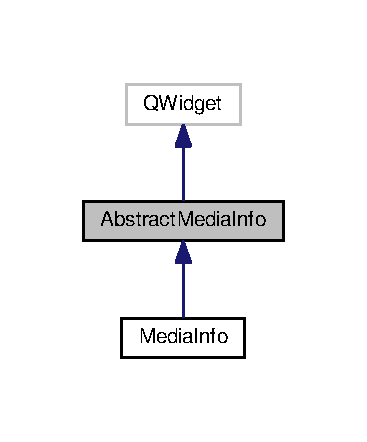
\includegraphics[width=176pt]{class_abstract_media_info__inherit__graph}
\end{center}
\end{figure}


Collaboration diagram for Abstract\-Media\-Info\-:
\nopagebreak
\begin{figure}[H]
\begin{center}
\leavevmode
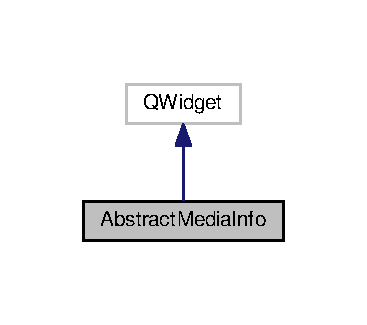
\includegraphics[width=176pt]{class_abstract_media_info__coll__graph}
\end{center}
\end{figure}
\subsection*{Public Slots}
\begin{DoxyCompactItemize}
\item 
\hypertarget{class_abstract_media_info_a59e096003b04baa551608fba8bed00d1}{virtual void {\bfseries set\-Atribute} (Q\-String property, Q\-String value)=0}\label{class_abstract_media_info_a59e096003b04baa551608fba8bed00d1}

\end{DoxyCompactItemize}
\subsection*{Public Member Functions}
\begin{DoxyCompactItemize}
\item 
\hypertarget{class_abstract_media_info_a9e2f1e341c8be06217de939859c93045}{{\bfseries Abstract\-Media\-Info} (Q\-Widget $\ast$parent=0)}\label{class_abstract_media_info_a9e2f1e341c8be06217de939859c93045}

\end{DoxyCompactItemize}


The documentation for this class was generated from the following file\-:\begin{DoxyCompactItemize}
\item 
abstractmediainfo.\-h\end{DoxyCompactItemize}

\hypertarget{class_abstract_spectrograph}{\section{Referência à classe Abstract\-Spectrograph}
\label{class_abstract_spectrograph}\index{Abstract\-Spectrograph@{Abstract\-Spectrograph}}
}
Diagrama de heranças da classe Abstract\-Spectrograph\begin{figure}[H]
\begin{center}
\leavevmode
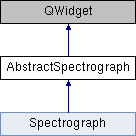
\includegraphics[height=3.000000cm]{class_abstract_spectrograph}
\end{center}
\end{figure}
\subsection*{Slots públicos}
\begin{DoxyCompactItemize}
\item 
\hypertarget{class_abstract_spectrograph_a63839b1e9464f8000a9469f013a6e30c}{virtual void {\bfseries load\-Samples} (Q\-Vector$<$ double $>$ \&)=0}\label{class_abstract_spectrograph_a63839b1e9464f8000a9469f013a6e30c}

\item 
\hypertarget{class_abstract_spectrograph_a04da5584e18bbd8954d9daef88418daa}{virtual void {\bfseries load\-Levels} (double, double)=0}\label{class_abstract_spectrograph_a04da5584e18bbd8954d9daef88418daa}

\end{DoxyCompactItemize}
\subsection*{Membros públicos}
\begin{DoxyCompactItemize}
\item 
\hypertarget{class_abstract_spectrograph_a623904d57582b553e0c15005a3690fd0}{{\bfseries Abstract\-Spectrograph} (Q\-Widget $\ast$)}\label{class_abstract_spectrograph_a623904d57582b553e0c15005a3690fd0}

\end{DoxyCompactItemize}


A documentação para esta classe foi gerada a partir do seguinte ficheiro\-:\begin{DoxyCompactItemize}
\item 
abstractspectrograph.\-h\end{DoxyCompactItemize}

\hypertarget{class_buffer_processor}{\section{Buffer\-Processor Class Reference}
\label{class_buffer_processor}\index{Buffer\-Processor@{Buffer\-Processor}}
}


{\ttfamily \#include $<$fftcalc.\-h$>$}

Inheritance diagram for Buffer\-Processor\-:\begin{figure}[H]
\begin{center}
\leavevmode
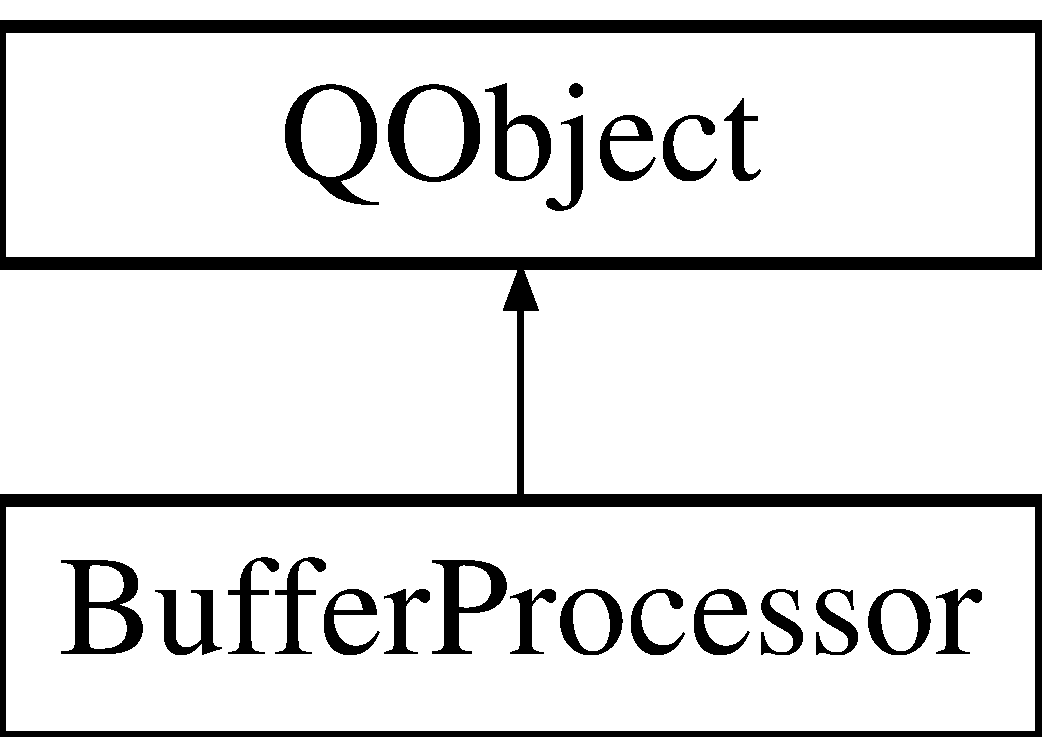
\includegraphics[height=2.000000cm]{class_buffer_processor}
\end{center}
\end{figure}
\subsection*{Public Slots}
\begin{DoxyCompactItemize}
\item 
void \hyperlink{class_buffer_processor_a19fedc34939ba4579b9a9bc3c53b7503}{process\-Buffer} (Q\-Vector$<$ double $>$ \-\_\-array, int duration)
\end{DoxyCompactItemize}
\subsection*{Signals}
\begin{DoxyCompactItemize}
\item 
void \hyperlink{class_buffer_processor_a466db3cca5282cd8b1d8c2ad6289ba35}{calculated\-Spectrum} (Q\-Vector$<$ double $>$ spectrum)
\item 
void \hyperlink{class_buffer_processor_a9dd9e6636e0dc2a4a263f045a3338013}{all\-Done} (void)
\end{DoxyCompactItemize}
\subsection*{Public Member Functions}
\begin{DoxyCompactItemize}
\item 
\hyperlink{class_buffer_processor_a910d84b159f28bcaf05b47ce7e81eb0c}{Buffer\-Processor} (Q\-Object $\ast$parent=0)
\item 
\hyperlink{class_buffer_processor_a3bff89bec0e670f7ae5386bfa7937401}{$\sim$\-Buffer\-Processor} ()
\item 
void \hyperlink{class_buffer_processor_af90a936a161872a0a4d4406af2822db9}{calc} (Q\-Vector$<$ double $>$ \&\-\_\-array, int duration)
\end{DoxyCompactItemize}
\subsection*{Protected Slots}
\begin{DoxyCompactItemize}
\item 
void \hyperlink{class_buffer_processor_a6faf10ab214287a399d05fce676dca6e}{run} ()
\end{DoxyCompactItemize}


\subsection{Constructor \& Destructor Documentation}
\hypertarget{class_buffer_processor_a910d84b159f28bcaf05b47ce7e81eb0c}{\index{Buffer\-Processor@{Buffer\-Processor}!Buffer\-Processor@{Buffer\-Processor}}
\index{Buffer\-Processor@{Buffer\-Processor}!BufferProcessor@{Buffer\-Processor}}
\subsubsection[{Buffer\-Processor}]{\setlength{\rightskip}{0pt plus 5cm}Buffer\-Processor\-::\-Buffer\-Processor (
\begin{DoxyParamCaption}
\item[{Q\-Object $\ast$}]{parent = {\ttfamily 0}}
\end{DoxyParamCaption}
)\hspace{0.3cm}{\ttfamily [explicit]}}}\label{class_buffer_processor_a910d84b159f28bcaf05b47ce7e81eb0c}
\hypertarget{class_buffer_processor_a3bff89bec0e670f7ae5386bfa7937401}{\index{Buffer\-Processor@{Buffer\-Processor}!$\sim$\-Buffer\-Processor@{$\sim$\-Buffer\-Processor}}
\index{$\sim$\-Buffer\-Processor@{$\sim$\-Buffer\-Processor}!BufferProcessor@{Buffer\-Processor}}
\subsubsection[{$\sim$\-Buffer\-Processor}]{\setlength{\rightskip}{0pt plus 5cm}Buffer\-Processor\-::$\sim$\-Buffer\-Processor (
\begin{DoxyParamCaption}
{}
\end{DoxyParamCaption}
)}}\label{class_buffer_processor_a3bff89bec0e670f7ae5386bfa7937401}


\subsection{Member Function Documentation}
\hypertarget{class_buffer_processor_a9dd9e6636e0dc2a4a263f045a3338013}{\index{Buffer\-Processor@{Buffer\-Processor}!all\-Done@{all\-Done}}
\index{all\-Done@{all\-Done}!BufferProcessor@{Buffer\-Processor}}
\subsubsection[{all\-Done}]{\setlength{\rightskip}{0pt plus 5cm}void Buffer\-Processor\-::all\-Done (
\begin{DoxyParamCaption}
\item[{void}]{}
\end{DoxyParamCaption}
)\hspace{0.3cm}{\ttfamily [signal]}}}\label{class_buffer_processor_a9dd9e6636e0dc2a4a263f045a3338013}
\hypertarget{class_buffer_processor_af90a936a161872a0a4d4406af2822db9}{\index{Buffer\-Processor@{Buffer\-Processor}!calc@{calc}}
\index{calc@{calc}!BufferProcessor@{Buffer\-Processor}}
\subsubsection[{calc}]{\setlength{\rightskip}{0pt plus 5cm}void Buffer\-Processor\-::calc (
\begin{DoxyParamCaption}
\item[{Q\-Vector$<$ double $>$ \&}]{\-\_\-array, }
\item[{int}]{duration}
\end{DoxyParamCaption}
)}}\label{class_buffer_processor_af90a936a161872a0a4d4406af2822db9}
\hypertarget{class_buffer_processor_a466db3cca5282cd8b1d8c2ad6289ba35}{\index{Buffer\-Processor@{Buffer\-Processor}!calculated\-Spectrum@{calculated\-Spectrum}}
\index{calculated\-Spectrum@{calculated\-Spectrum}!BufferProcessor@{Buffer\-Processor}}
\subsubsection[{calculated\-Spectrum}]{\setlength{\rightskip}{0pt plus 5cm}void Buffer\-Processor\-::calculated\-Spectrum (
\begin{DoxyParamCaption}
\item[{Q\-Vector$<$ double $>$}]{spectrum}
\end{DoxyParamCaption}
)\hspace{0.3cm}{\ttfamily [signal]}}}\label{class_buffer_processor_a466db3cca5282cd8b1d8c2ad6289ba35}
\hypertarget{class_buffer_processor_a19fedc34939ba4579b9a9bc3c53b7503}{\index{Buffer\-Processor@{Buffer\-Processor}!process\-Buffer@{process\-Buffer}}
\index{process\-Buffer@{process\-Buffer}!BufferProcessor@{Buffer\-Processor}}
\subsubsection[{process\-Buffer}]{\setlength{\rightskip}{0pt plus 5cm}void Buffer\-Processor\-::process\-Buffer (
\begin{DoxyParamCaption}
\item[{Q\-Vector$<$ double $>$}]{\-\_\-array, }
\item[{int}]{duration}
\end{DoxyParamCaption}
)\hspace{0.3cm}{\ttfamily [slot]}}}\label{class_buffer_processor_a19fedc34939ba4579b9a9bc3c53b7503}
\hypertarget{class_buffer_processor_a6faf10ab214287a399d05fce676dca6e}{\index{Buffer\-Processor@{Buffer\-Processor}!run@{run}}
\index{run@{run}!BufferProcessor@{Buffer\-Processor}}
\subsubsection[{run}]{\setlength{\rightskip}{0pt plus 5cm}void Buffer\-Processor\-::run (
\begin{DoxyParamCaption}
{}
\end{DoxyParamCaption}
)\hspace{0.3cm}{\ttfamily [protected]}, {\ttfamily [slot]}}}\label{class_buffer_processor_a6faf10ab214287a399d05fce676dca6e}


The documentation for this class was generated from the following files\-:\begin{DoxyCompactItemize}
\item 
\hyperlink{fftcalc_8h}{fftcalc.\-h}\item 
\hyperlink{fftcalc_8cpp}{fftcalc.\-cpp}\end{DoxyCompactItemize}

\hypertarget{class_controls}{\section{Referência à classe Controls}
\label{class_controls}\index{Controls@{Controls}}
}
Diagrama de heranças da classe Controls\begin{figure}[H]
\begin{center}
\leavevmode
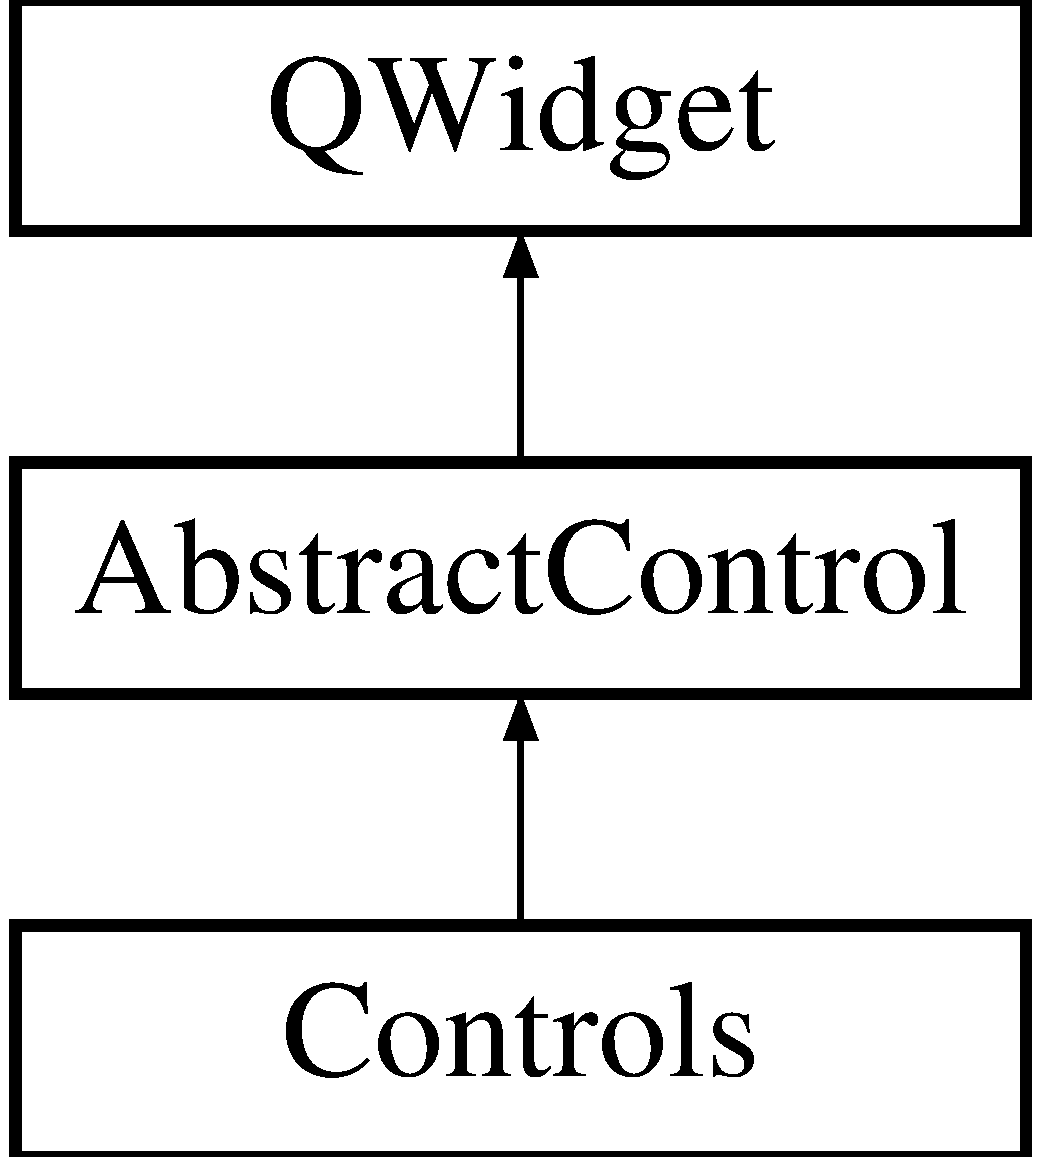
\includegraphics[height=3.000000cm]{class_controls}
\end{center}
\end{figure}
\subsection*{Slots públicos}
\begin{DoxyCompactItemize}
\item 
\hypertarget{class_controls_ae5e221035bf36156c77c629fe4be453d}{void {\bfseries on\-Play\-Pause\-Clicked} (void)}\label{class_controls_ae5e221035bf36156c77c629fe4be453d}

\item 
\hypertarget{class_controls_a48610eb52367be6c7509457244821335}{void {\bfseries on\-Prev\-Clicked} (void)}\label{class_controls_a48610eb52367be6c7509457244821335}

\item 
\hypertarget{class_controls_a4e7c1ea477ffeb066399d48404ede8b0}{void {\bfseries on\-Next\-Clicked} (void)}\label{class_controls_a4e7c1ea477ffeb066399d48404ede8b0}

\item 
\hypertarget{class_controls_af599078654027314f33d922ce601a054}{void {\bfseries on\-Volume\-Changed} (int value)}\label{class_controls_af599078654027314f33d922ce601a054}

\item 
\hypertarget{class_controls_a09f5f92331f2531ead8a02612ae60127}{void {\bfseries on\-Elapsed\-Changed} (qint64 value)}\label{class_controls_a09f5f92331f2531ead8a02612ae60127}

\item 
\hypertarget{class_controls_a7abbbb170c237e803401311c012492ba}{void {\bfseries on\-Duration\-Changed} (qint64 value)}\label{class_controls_a7abbbb170c237e803401311c012492ba}

\end{DoxyCompactItemize}
\subsection*{Sinais}
\begin{DoxyCompactItemize}
\item 
\hypertarget{class_controls_afe7504ad0f381214c4183e5be814abc4}{void {\bfseries play\-Pause} ()}\label{class_controls_afe7504ad0f381214c4183e5be814abc4}

\item 
\hypertarget{class_controls_af74535d8202bfdb9049eb58f7d13e690}{void {\bfseries next} ()}\label{class_controls_af74535d8202bfdb9049eb58f7d13e690}

\item 
\hypertarget{class_controls_a166980f14fdc874aecbd5b96ee631888}{void {\bfseries prev} ()}\label{class_controls_a166980f14fdc874aecbd5b96ee631888}

\item 
\hypertarget{class_controls_abcd261c1a0fe72dc44eb49bebbe0931a}{void {\bfseries stop} ()}\label{class_controls_abcd261c1a0fe72dc44eb49bebbe0931a}

\item 
\hypertarget{class_controls_ab4219d5113b05a478c25c5c41203eaf7}{void {\bfseries volume\-Selected} (int)}\label{class_controls_ab4219d5113b05a478c25c5c41203eaf7}

\item 
\hypertarget{class_controls_ac44bbe30565ace7514dbb2d0337419a6}{void {\bfseries elapsed\-Selected} (qint64)}\label{class_controls_ac44bbe30565ace7514dbb2d0337419a6}

\end{DoxyCompactItemize}
\subsection*{Membros públicos}
\begin{DoxyCompactItemize}
\item 
\hypertarget{class_controls_a1f825cd40c51b25d483e5c11f052737c}{{\bfseries Controls} (Q\-Widget $\ast$parent=0)}\label{class_controls_a1f825cd40c51b25d483e5c11f052737c}

\end{DoxyCompactItemize}
\subsection*{Slots protegidos}
\begin{DoxyCompactItemize}
\item 
\hypertarget{class_controls_a45ba0a2beabcacf2065807adce607e73}{void {\bfseries on\-Slider\-Released} ()}\label{class_controls_a45ba0a2beabcacf2065807adce607e73}

\end{DoxyCompactItemize}


A documentação para esta classe foi gerada a partir dos seguintes ficheiros\-:\begin{DoxyCompactItemize}
\item 
controls.\-h\item 
controls.\-cpp\end{DoxyCompactItemize}

\hypertarget{class_f_f_t_calc}{\section{Referência à classe F\-F\-T\-Calc}
\label{class_f_f_t_calc}\index{F\-F\-T\-Calc@{F\-F\-T\-Calc}}
}
Diagrama de heranças da classe F\-F\-T\-Calc\begin{figure}[H]
\begin{center}
\leavevmode
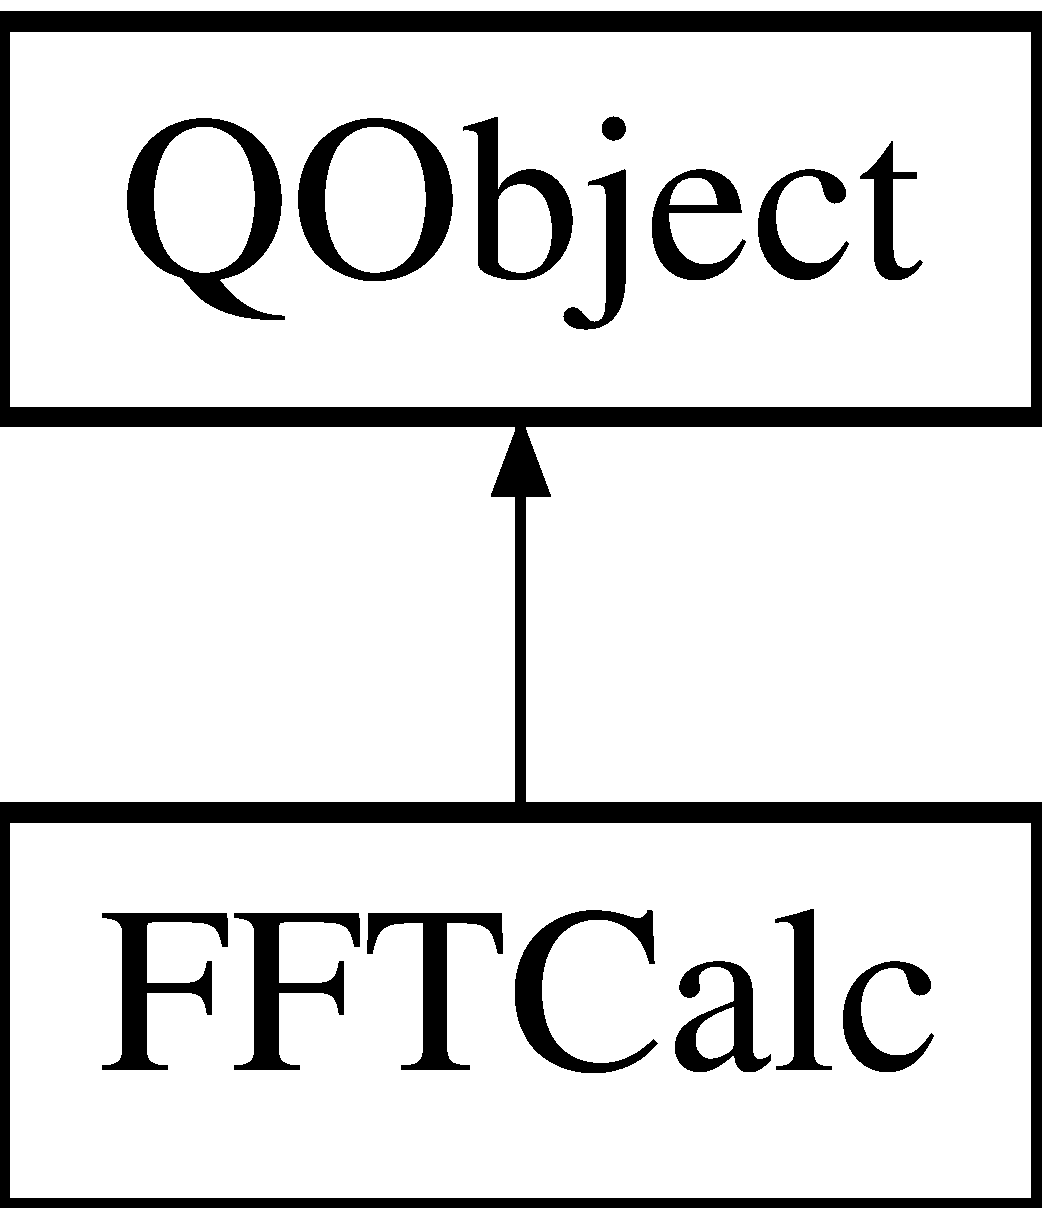
\includegraphics[height=2.000000cm]{class_f_f_t_calc}
\end{center}
\end{figure}
\subsection*{Slots públicos}
\begin{DoxyCompactItemize}
\item 
\hypertarget{class_f_f_t_calc_a630f0941389aa764c341c15a50d6c51a}{void {\bfseries set\-Spectrum} (Q\-Vector$<$ double $>$ spectrum)}\label{class_f_f_t_calc_a630f0941389aa764c341c15a50d6c51a}

\item 
\hypertarget{class_f_f_t_calc_ae12ef5c098a2bb3070a743927ef50da7}{void {\bfseries free\-Calc} ()}\label{class_f_f_t_calc_ae12ef5c098a2bb3070a743927ef50da7}

\end{DoxyCompactItemize}
\subsection*{Sinais}
\begin{DoxyCompactItemize}
\item 
\hypertarget{class_f_f_t_calc_a2c21488cc4fa4985f9152156137db30e}{void {\bfseries calculated\-Spectrum} (Q\-Vector$<$ double $>$ spectrum)}\label{class_f_f_t_calc_a2c21488cc4fa4985f9152156137db30e}

\end{DoxyCompactItemize}
\subsection*{Membros públicos}
\begin{DoxyCompactItemize}
\item 
\hypertarget{class_f_f_t_calc_ae6b220dd66a6df99041680e55746c79e}{{\bfseries F\-F\-T\-Calc} (Q\-Object $\ast$parent=0)}\label{class_f_f_t_calc_ae6b220dd66a6df99041680e55746c79e}

\item 
\hypertarget{class_f_f_t_calc_a19ee0f470123aaff939fc6c1ee833080}{void {\bfseries calc} (Q\-Vector$<$ double $>$ \&\-\_\-array, int duration)}\label{class_f_f_t_calc_a19ee0f470123aaff939fc6c1ee833080}

\end{DoxyCompactItemize}


A documentação para esta classe foi gerada a partir dos seguintes ficheiros\-:\begin{DoxyCompactItemize}
\item 
fftcalc.\-h\item 
fftcalc.\-cpp\end{DoxyCompactItemize}

\hypertarget{class_main_window}{\section{Main\-Window Class Reference}
\label{class_main_window}\index{Main\-Window@{Main\-Window}}
}


{\ttfamily \#include $<$mainwindow.\-h$>$}

Inheritance diagram for Main\-Window\-:\begin{figure}[H]
\begin{center}
\leavevmode
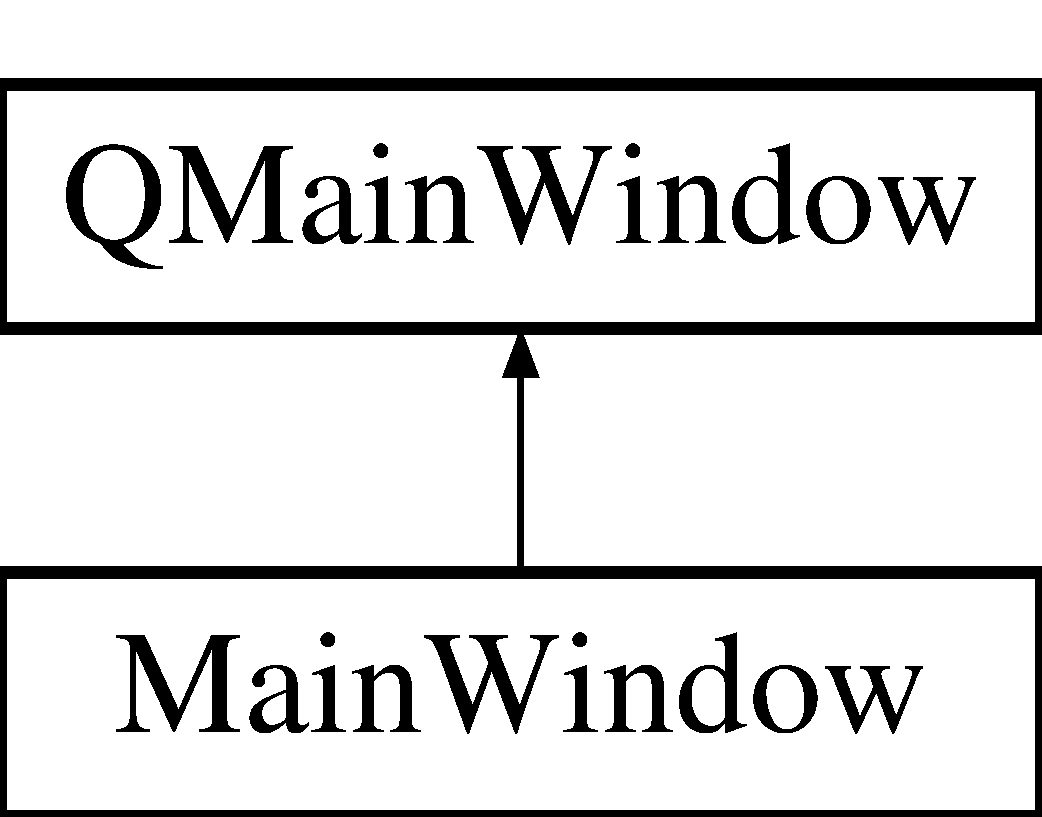
\includegraphics[height=2.000000cm]{class_main_window}
\end{center}
\end{figure}
\subsection*{Public Slots}
\begin{DoxyCompactItemize}
\item 
void \hyperlink{class_main_window_a32e621ebdb3ef2d76bd607af16e8d0d0}{go\-To\-Item} (const Q\-Model\-Index \&index)
\item 
void \hyperlink{class_main_window_a5dc0f9a967ac6c534cfbf6e517275ba9}{load\-Media} ()
\item 
void \hyperlink{class_main_window_ac877ae03abf6415808e0bb36ff71e5be}{load\-Playlist} ()
\item 
void \hyperlink{class_main_window_a8bb0a943725aa0d7959a8a93da3194fc}{on\-Add\-Media\-To\-Play\-List} (Q\-String media)
\item 
void \hyperlink{class_main_window_a2758962312cc237231c349b21603d9fe}{media\-Status\-Changed} (Q\-Media\-Player\-::\-Media\-Status status)
\item 
void \hyperlink{class_main_window_aa4ec6868c3ee50f63ffe4803a7136ae6}{meta\-Data\-Changed} ()
\item 
void \hyperlink{class_main_window_aabed273350d064a3a8d73afb01848fea}{next} ()
\item 
void \hyperlink{class_main_window_a6e12ed66de9615bf272f92a47cd5e6c8}{play\-Pause} ()
\item 
void \hyperlink{class_main_window_a44f59c80c2093aaaca31cfc82def698f}{slot\-Position\-Changed} (qint64 e)
\item 
void \hyperlink{class_main_window_a56270e72e4ec5e058a040657932069cf}{prev} ()
\item 
void \hyperlink{class_main_window_a5c459d00d64786ef93db7670034af47d}{process\-Buffer} (Q\-Audio\-Buffer buffer)
\item 
void \hyperlink{class_main_window_aedb83314811efab4ea67c69cbce29aea}{set\-Media\-At} (qint32 percent)
\item 
void \hyperlink{class_main_window_aeb9309a7fe8efd574fe5b7ac92ba2a92}{set\-Volume} (int volume)
\item 
void \hyperlink{class_main_window_a9efd699e3eaed3396733475499297bc0}{spectrum\-Available} (Q\-Vector$<$ double $>$ spectrum)
\item 
void \hyperlink{class_main_window_ac7664400c470d7312a62ec8f4f7822a6}{meta\-Data\-Available\-Changed} (bool)
\end{DoxyCompactItemize}
\subsection*{Signals}
\begin{DoxyCompactItemize}
\item 
int \hyperlink{class_main_window_a0db59b0091efb9ef939245562e84b79a}{spectrum\-Changed} (Q\-Vector$<$ double $>$ \&sample)
\item 
int \hyperlink{class_main_window_a8df9e5e5d0997eb8e5ecdbcf42bb57ca}{position\-Changed} (qint64 position)
\item 
int \hyperlink{class_main_window_a59803bb114724dc5f3717dc28539f164}{levels} (double left, double right)
\item 
int \hyperlink{class_main_window_ad255b6b8019a66a663a9c1de04d42a80}{elapsed\-Time\-Changed} (qint64 elapsed)
\item 
int \hyperlink{class_main_window_a659d33ceffcceae28005205fe44edda4}{add\-Folder\-To\-Library} (Q\-String folder)
\end{DoxyCompactItemize}
\subsection*{Public Member Functions}
\begin{DoxyCompactItemize}
\item 
\hyperlink{class_main_window_a8b244be8b7b7db1b08de2a2acb9409db}{Main\-Window} (Q\-Widget $\ast$parent=0)
\item 
\hyperlink{class_main_window_ae98d00a93bc118200eeef9f9bba1dba7}{$\sim$\-Main\-Window} ()
\end{DoxyCompactItemize}


\subsection{Constructor \& Destructor Documentation}
\hypertarget{class_main_window_a8b244be8b7b7db1b08de2a2acb9409db}{\index{Main\-Window@{Main\-Window}!Main\-Window@{Main\-Window}}
\index{Main\-Window@{Main\-Window}!MainWindow@{Main\-Window}}
\subsubsection[{Main\-Window}]{\setlength{\rightskip}{0pt plus 5cm}Main\-Window\-::\-Main\-Window (
\begin{DoxyParamCaption}
\item[{Q\-Widget $\ast$}]{parent = {\ttfamily 0}}
\end{DoxyParamCaption}
)\hspace{0.3cm}{\ttfamily [explicit]}}}\label{class_main_window_a8b244be8b7b7db1b08de2a2acb9409db}
\hypertarget{class_main_window_ae98d00a93bc118200eeef9f9bba1dba7}{\index{Main\-Window@{Main\-Window}!$\sim$\-Main\-Window@{$\sim$\-Main\-Window}}
\index{$\sim$\-Main\-Window@{$\sim$\-Main\-Window}!MainWindow@{Main\-Window}}
\subsubsection[{$\sim$\-Main\-Window}]{\setlength{\rightskip}{0pt plus 5cm}Main\-Window\-::$\sim$\-Main\-Window (
\begin{DoxyParamCaption}
{}
\end{DoxyParamCaption}
)}}\label{class_main_window_ae98d00a93bc118200eeef9f9bba1dba7}


\subsection{Member Function Documentation}
\hypertarget{class_main_window_a659d33ceffcceae28005205fe44edda4}{\index{Main\-Window@{Main\-Window}!add\-Folder\-To\-Library@{add\-Folder\-To\-Library}}
\index{add\-Folder\-To\-Library@{add\-Folder\-To\-Library}!MainWindow@{Main\-Window}}
\subsubsection[{add\-Folder\-To\-Library}]{\setlength{\rightskip}{0pt plus 5cm}int Main\-Window\-::add\-Folder\-To\-Library (
\begin{DoxyParamCaption}
\item[{Q\-String}]{folder}
\end{DoxyParamCaption}
)\hspace{0.3cm}{\ttfamily [signal]}}}\label{class_main_window_a659d33ceffcceae28005205fe44edda4}
\hypertarget{class_main_window_ad255b6b8019a66a663a9c1de04d42a80}{\index{Main\-Window@{Main\-Window}!elapsed\-Time\-Changed@{elapsed\-Time\-Changed}}
\index{elapsed\-Time\-Changed@{elapsed\-Time\-Changed}!MainWindow@{Main\-Window}}
\subsubsection[{elapsed\-Time\-Changed}]{\setlength{\rightskip}{0pt plus 5cm}int Main\-Window\-::elapsed\-Time\-Changed (
\begin{DoxyParamCaption}
\item[{qint64}]{elapsed}
\end{DoxyParamCaption}
)\hspace{0.3cm}{\ttfamily [signal]}}}\label{class_main_window_ad255b6b8019a66a663a9c1de04d42a80}
\hypertarget{class_main_window_a32e621ebdb3ef2d76bd607af16e8d0d0}{\index{Main\-Window@{Main\-Window}!go\-To\-Item@{go\-To\-Item}}
\index{go\-To\-Item@{go\-To\-Item}!MainWindow@{Main\-Window}}
\subsubsection[{go\-To\-Item}]{\setlength{\rightskip}{0pt plus 5cm}void Main\-Window\-::go\-To\-Item (
\begin{DoxyParamCaption}
\item[{const Q\-Model\-Index \&}]{index}
\end{DoxyParamCaption}
)\hspace{0.3cm}{\ttfamily [slot]}}}\label{class_main_window_a32e621ebdb3ef2d76bd607af16e8d0d0}
\hypertarget{class_main_window_a59803bb114724dc5f3717dc28539f164}{\index{Main\-Window@{Main\-Window}!levels@{levels}}
\index{levels@{levels}!MainWindow@{Main\-Window}}
\subsubsection[{levels}]{\setlength{\rightskip}{0pt plus 5cm}int Main\-Window\-::levels (
\begin{DoxyParamCaption}
\item[{double}]{left, }
\item[{double}]{right}
\end{DoxyParamCaption}
)\hspace{0.3cm}{\ttfamily [signal]}}}\label{class_main_window_a59803bb114724dc5f3717dc28539f164}
\hypertarget{class_main_window_a5dc0f9a967ac6c534cfbf6e517275ba9}{\index{Main\-Window@{Main\-Window}!load\-Media@{load\-Media}}
\index{load\-Media@{load\-Media}!MainWindow@{Main\-Window}}
\subsubsection[{load\-Media}]{\setlength{\rightskip}{0pt plus 5cm}void Main\-Window\-::load\-Media (
\begin{DoxyParamCaption}
{}
\end{DoxyParamCaption}
)\hspace{0.3cm}{\ttfamily [slot]}}}\label{class_main_window_a5dc0f9a967ac6c534cfbf6e517275ba9}
\hypertarget{class_main_window_ac877ae03abf6415808e0bb36ff71e5be}{\index{Main\-Window@{Main\-Window}!load\-Playlist@{load\-Playlist}}
\index{load\-Playlist@{load\-Playlist}!MainWindow@{Main\-Window}}
\subsubsection[{load\-Playlist}]{\setlength{\rightskip}{0pt plus 5cm}void Main\-Window\-::load\-Playlist (
\begin{DoxyParamCaption}
\item[{void}]{}
\end{DoxyParamCaption}
)\hspace{0.3cm}{\ttfamily [slot]}}}\label{class_main_window_ac877ae03abf6415808e0bb36ff71e5be}
\hypertarget{class_main_window_a2758962312cc237231c349b21603d9fe}{\index{Main\-Window@{Main\-Window}!media\-Status\-Changed@{media\-Status\-Changed}}
\index{media\-Status\-Changed@{media\-Status\-Changed}!MainWindow@{Main\-Window}}
\subsubsection[{media\-Status\-Changed}]{\setlength{\rightskip}{0pt plus 5cm}void Main\-Window\-::media\-Status\-Changed (
\begin{DoxyParamCaption}
\item[{Q\-Media\-Player\-::\-Media\-Status}]{status}
\end{DoxyParamCaption}
)\hspace{0.3cm}{\ttfamily [slot]}}}\label{class_main_window_a2758962312cc237231c349b21603d9fe}
\hypertarget{class_main_window_ac7664400c470d7312a62ec8f4f7822a6}{\index{Main\-Window@{Main\-Window}!meta\-Data\-Available\-Changed@{meta\-Data\-Available\-Changed}}
\index{meta\-Data\-Available\-Changed@{meta\-Data\-Available\-Changed}!MainWindow@{Main\-Window}}
\subsubsection[{meta\-Data\-Available\-Changed}]{\setlength{\rightskip}{0pt plus 5cm}void Main\-Window\-::meta\-Data\-Available\-Changed (
\begin{DoxyParamCaption}
\item[{bool}]{flag}
\end{DoxyParamCaption}
)\hspace{0.3cm}{\ttfamily [slot]}}}\label{class_main_window_ac7664400c470d7312a62ec8f4f7822a6}
\hypertarget{class_main_window_aa4ec6868c3ee50f63ffe4803a7136ae6}{\index{Main\-Window@{Main\-Window}!meta\-Data\-Changed@{meta\-Data\-Changed}}
\index{meta\-Data\-Changed@{meta\-Data\-Changed}!MainWindow@{Main\-Window}}
\subsubsection[{meta\-Data\-Changed}]{\setlength{\rightskip}{0pt plus 5cm}void Main\-Window\-::meta\-Data\-Changed (
\begin{DoxyParamCaption}
{}
\end{DoxyParamCaption}
)\hspace{0.3cm}{\ttfamily [slot]}}}\label{class_main_window_aa4ec6868c3ee50f63ffe4803a7136ae6}
\hypertarget{class_main_window_aabed273350d064a3a8d73afb01848fea}{\index{Main\-Window@{Main\-Window}!next@{next}}
\index{next@{next}!MainWindow@{Main\-Window}}
\subsubsection[{next}]{\setlength{\rightskip}{0pt plus 5cm}void Main\-Window\-::next (
\begin{DoxyParamCaption}
{}
\end{DoxyParamCaption}
)\hspace{0.3cm}{\ttfamily [slot]}}}\label{class_main_window_aabed273350d064a3a8d73afb01848fea}
\hypertarget{class_main_window_a8bb0a943725aa0d7959a8a93da3194fc}{\index{Main\-Window@{Main\-Window}!on\-Add\-Media\-To\-Play\-List@{on\-Add\-Media\-To\-Play\-List}}
\index{on\-Add\-Media\-To\-Play\-List@{on\-Add\-Media\-To\-Play\-List}!MainWindow@{Main\-Window}}
\subsubsection[{on\-Add\-Media\-To\-Play\-List}]{\setlength{\rightskip}{0pt plus 5cm}void Main\-Window\-::on\-Add\-Media\-To\-Play\-List (
\begin{DoxyParamCaption}
\item[{Q\-String}]{media}
\end{DoxyParamCaption}
)\hspace{0.3cm}{\ttfamily [slot]}}}\label{class_main_window_a8bb0a943725aa0d7959a8a93da3194fc}
\hypertarget{class_main_window_a6e12ed66de9615bf272f92a47cd5e6c8}{\index{Main\-Window@{Main\-Window}!play\-Pause@{play\-Pause}}
\index{play\-Pause@{play\-Pause}!MainWindow@{Main\-Window}}
\subsubsection[{play\-Pause}]{\setlength{\rightskip}{0pt plus 5cm}void Main\-Window\-::play\-Pause (
\begin{DoxyParamCaption}
{}
\end{DoxyParamCaption}
)\hspace{0.3cm}{\ttfamily [slot]}}}\label{class_main_window_a6e12ed66de9615bf272f92a47cd5e6c8}
\hypertarget{class_main_window_a8df9e5e5d0997eb8e5ecdbcf42bb57ca}{\index{Main\-Window@{Main\-Window}!position\-Changed@{position\-Changed}}
\index{position\-Changed@{position\-Changed}!MainWindow@{Main\-Window}}
\subsubsection[{position\-Changed}]{\setlength{\rightskip}{0pt plus 5cm}int Main\-Window\-::position\-Changed (
\begin{DoxyParamCaption}
\item[{qint64}]{position}
\end{DoxyParamCaption}
)\hspace{0.3cm}{\ttfamily [signal]}}}\label{class_main_window_a8df9e5e5d0997eb8e5ecdbcf42bb57ca}
\hypertarget{class_main_window_a56270e72e4ec5e058a040657932069cf}{\index{Main\-Window@{Main\-Window}!prev@{prev}}
\index{prev@{prev}!MainWindow@{Main\-Window}}
\subsubsection[{prev}]{\setlength{\rightskip}{0pt plus 5cm}void Main\-Window\-::prev (
\begin{DoxyParamCaption}
{}
\end{DoxyParamCaption}
)\hspace{0.3cm}{\ttfamily [slot]}}}\label{class_main_window_a56270e72e4ec5e058a040657932069cf}
\hypertarget{class_main_window_a5c459d00d64786ef93db7670034af47d}{\index{Main\-Window@{Main\-Window}!process\-Buffer@{process\-Buffer}}
\index{process\-Buffer@{process\-Buffer}!MainWindow@{Main\-Window}}
\subsubsection[{process\-Buffer}]{\setlength{\rightskip}{0pt plus 5cm}void Main\-Window\-::process\-Buffer (
\begin{DoxyParamCaption}
\item[{Q\-Audio\-Buffer}]{buffer}
\end{DoxyParamCaption}
)\hspace{0.3cm}{\ttfamily [slot]}}}\label{class_main_window_a5c459d00d64786ef93db7670034af47d}
\hypertarget{class_main_window_aedb83314811efab4ea67c69cbce29aea}{\index{Main\-Window@{Main\-Window}!set\-Media\-At@{set\-Media\-At}}
\index{set\-Media\-At@{set\-Media\-At}!MainWindow@{Main\-Window}}
\subsubsection[{set\-Media\-At}]{\setlength{\rightskip}{0pt plus 5cm}void Main\-Window\-::set\-Media\-At (
\begin{DoxyParamCaption}
\item[{qint32}]{percent}
\end{DoxyParamCaption}
)\hspace{0.3cm}{\ttfamily [slot]}}}\label{class_main_window_aedb83314811efab4ea67c69cbce29aea}
\hypertarget{class_main_window_aeb9309a7fe8efd574fe5b7ac92ba2a92}{\index{Main\-Window@{Main\-Window}!set\-Volume@{set\-Volume}}
\index{set\-Volume@{set\-Volume}!MainWindow@{Main\-Window}}
\subsubsection[{set\-Volume}]{\setlength{\rightskip}{0pt plus 5cm}void Main\-Window\-::set\-Volume (
\begin{DoxyParamCaption}
\item[{int}]{volume}
\end{DoxyParamCaption}
)\hspace{0.3cm}{\ttfamily [slot]}}}\label{class_main_window_aeb9309a7fe8efd574fe5b7ac92ba2a92}
\hypertarget{class_main_window_a44f59c80c2093aaaca31cfc82def698f}{\index{Main\-Window@{Main\-Window}!slot\-Position\-Changed@{slot\-Position\-Changed}}
\index{slot\-Position\-Changed@{slot\-Position\-Changed}!MainWindow@{Main\-Window}}
\subsubsection[{slot\-Position\-Changed}]{\setlength{\rightskip}{0pt plus 5cm}void Main\-Window\-::slot\-Position\-Changed (
\begin{DoxyParamCaption}
\item[{qint64}]{e}
\end{DoxyParamCaption}
)\hspace{0.3cm}{\ttfamily [slot]}}}\label{class_main_window_a44f59c80c2093aaaca31cfc82def698f}
\hypertarget{class_main_window_a9efd699e3eaed3396733475499297bc0}{\index{Main\-Window@{Main\-Window}!spectrum\-Available@{spectrum\-Available}}
\index{spectrum\-Available@{spectrum\-Available}!MainWindow@{Main\-Window}}
\subsubsection[{spectrum\-Available}]{\setlength{\rightskip}{0pt plus 5cm}void Main\-Window\-::spectrum\-Available (
\begin{DoxyParamCaption}
\item[{Q\-Vector$<$ double $>$}]{spectrum}
\end{DoxyParamCaption}
)\hspace{0.3cm}{\ttfamily [slot]}}}\label{class_main_window_a9efd699e3eaed3396733475499297bc0}
\hypertarget{class_main_window_a0db59b0091efb9ef939245562e84b79a}{\index{Main\-Window@{Main\-Window}!spectrum\-Changed@{spectrum\-Changed}}
\index{spectrum\-Changed@{spectrum\-Changed}!MainWindow@{Main\-Window}}
\subsubsection[{spectrum\-Changed}]{\setlength{\rightskip}{0pt plus 5cm}int Main\-Window\-::spectrum\-Changed (
\begin{DoxyParamCaption}
\item[{Q\-Vector$<$ double $>$ \&}]{sample}
\end{DoxyParamCaption}
)\hspace{0.3cm}{\ttfamily [signal]}}}\label{class_main_window_a0db59b0091efb9ef939245562e84b79a}


The documentation for this class was generated from the following files\-:\begin{DoxyCompactItemize}
\item 
\hyperlink{mainwindow_8h}{mainwindow.\-h}\item 
\hyperlink{mainwindow_8cpp}{mainwindow.\-cpp}\end{DoxyCompactItemize}

\hypertarget{class_media_info}{\section{Media\-Info Class Reference}
\label{class_media_info}\index{Media\-Info@{Media\-Info}}
}


Inheritance diagram for Media\-Info\-:
\nopagebreak
\begin{figure}[H]
\begin{center}
\leavevmode
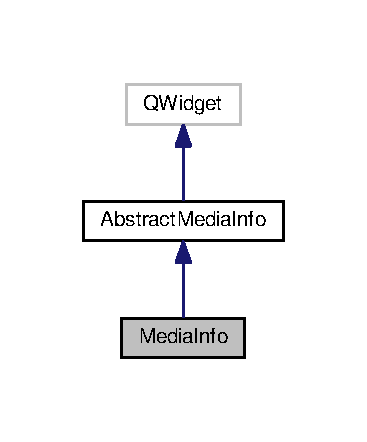
\includegraphics[width=176pt]{class_media_info__inherit__graph}
\end{center}
\end{figure}


Collaboration diagram for Media\-Info\-:
\nopagebreak
\begin{figure}[H]
\begin{center}
\leavevmode
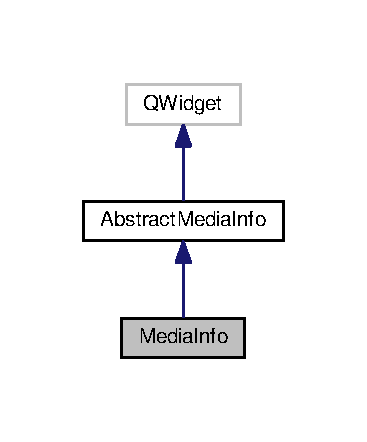
\includegraphics[width=176pt]{class_media_info__coll__graph}
\end{center}
\end{figure}
\subsection*{Public Slots}
\begin{DoxyCompactItemize}
\item 
\hypertarget{class_media_info_ac1a807582e0830e8f7a6167257a8b69a}{void {\bfseries set\-Atribute} (Q\-String property, Q\-String value)}\label{class_media_info_ac1a807582e0830e8f7a6167257a8b69a}

\end{DoxyCompactItemize}
\subsection*{Public Member Functions}
\begin{DoxyCompactItemize}
\item 
\hypertarget{class_media_info_a80b7af5a999c7ab31e4207c39ccb8833}{{\bfseries Media\-Info} (Q\-Widget $\ast$parent=0)}\label{class_media_info_a80b7af5a999c7ab31e4207c39ccb8833}

\end{DoxyCompactItemize}


The documentation for this class was generated from the following files\-:\begin{DoxyCompactItemize}
\item 
mediainfo.\-h\item 
mediainfo.\-cpp\end{DoxyCompactItemize}

\hypertarget{class_playlist_model}{\section{Playlist\-Model Class Reference}
\label{class_playlist_model}\index{Playlist\-Model@{Playlist\-Model}}
}


{\ttfamily \#include $<$playlistmodel.\-h$>$}

Inheritance diagram for Playlist\-Model\-:\begin{figure}[H]
\begin{center}
\leavevmode
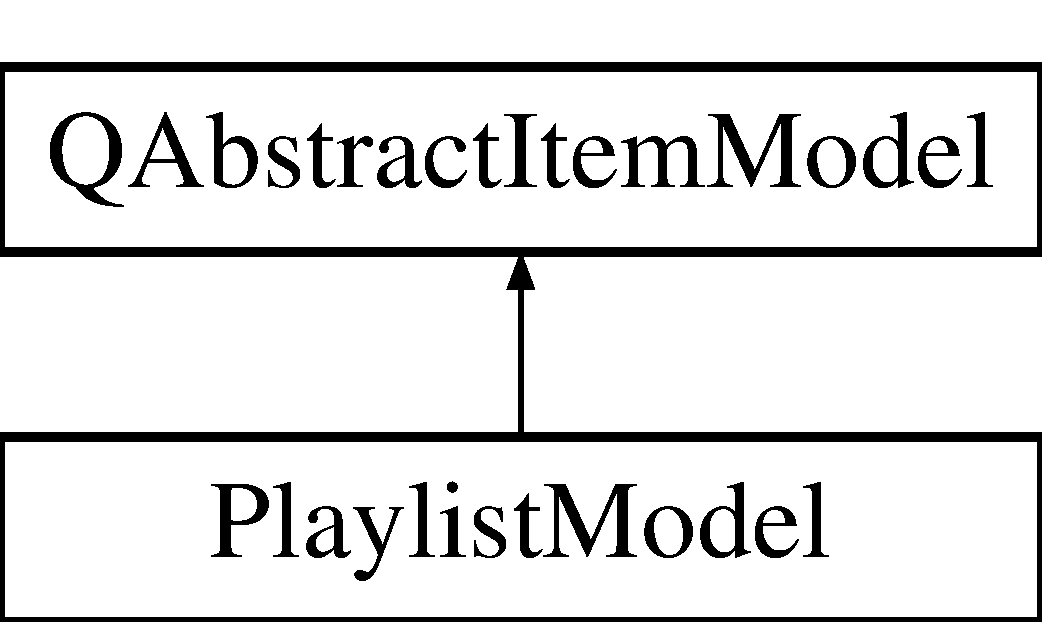
\includegraphics[height=2.000000cm]{class_playlist_model}
\end{center}
\end{figure}
\subsection*{Public Types}
\begin{DoxyCompactItemize}
\item 
enum \hyperlink{class_playlist_model_a85df23455e37bba0806ef488fb96f435}{Column} \{ \hyperlink{class_playlist_model_a85df23455e37bba0806ef488fb96f435ad177ef9079b494b37664af91083db9f2}{Title} = 0, 
\hyperlink{class_playlist_model_a85df23455e37bba0806ef488fb96f435a5e948ab2605fd6c754aff3bef76f0373}{Column\-Count}
 \}
\end{DoxyCompactItemize}
\subsection*{Public Slots}
\begin{DoxyCompactItemize}
\item 
int \hyperlink{class_playlist_model_a2deef5b14f8f66431a55fdb0484025b6}{row\-Count} (const Q\-Model\-Index \&\hyperlink{class_playlist_model_a8ff71ee8d706da034fbe8b9b613a940c}{parent}=Q\-Model\-Index()) const 
\item 
int \hyperlink{class_playlist_model_a50cd819e7dec4c4881eebaed8130944d}{column\-Count} (const Q\-Model\-Index \&\hyperlink{class_playlist_model_a8ff71ee8d706da034fbe8b9b613a940c}{parent}=Q\-Model\-Index()) const 
\item 
Q\-Model\-Index \hyperlink{class_playlist_model_a03d1879138b2a0c6c68d7f6d98cfa92a}{index} (int row, int column, const Q\-Model\-Index \&\hyperlink{class_playlist_model_a8ff71ee8d706da034fbe8b9b613a940c}{parent}=Q\-Model\-Index()) const 
\item 
Q\-Model\-Index \hyperlink{class_playlist_model_a8ff71ee8d706da034fbe8b9b613a940c}{parent} (const Q\-Model\-Index \&child) const 
\item 
Q\-Variant \hyperlink{class_playlist_model_ac3d2bee2441ad8d13662833fd5968aac}{data} (const Q\-Model\-Index \&\hyperlink{class_playlist_model_a03d1879138b2a0c6c68d7f6d98cfa92a}{index}, int role=Qt\-::\-Display\-Role) const 
\item 
Q\-Media\-Playlist $\ast$ \hyperlink{class_playlist_model_afe7dce718749f036b23a8cf749dc4388}{playlist} () const 
\item 
void \hyperlink{class_playlist_model_aaf551c97c7a8ded2a3d3333f15f558a5}{set\-Playlist} (Q\-Media\-Playlist $\ast$\hyperlink{class_playlist_model_afe7dce718749f036b23a8cf749dc4388}{playlist})
\item 
bool \hyperlink{class_playlist_model_a61fcc4b9d0eaad86492c283b05c30fbc}{set\-Data} (const Q\-Model\-Index \&\hyperlink{class_playlist_model_a03d1879138b2a0c6c68d7f6d98cfa92a}{index}, const Q\-Variant \&value, int role=Qt\-::\-Display\-Role)
\end{DoxyCompactItemize}
\subsection*{Public Member Functions}
\begin{DoxyCompactItemize}
\item 
\hyperlink{class_playlist_model_a62aaf86821f96310da890e94ff083cb8}{Playlist\-Model} (Q\-Object $\ast$\hyperlink{class_playlist_model_a8ff71ee8d706da034fbe8b9b613a940c}{parent}=0)
\end{DoxyCompactItemize}


\subsection{Member Enumeration Documentation}
\hypertarget{class_playlist_model_a85df23455e37bba0806ef488fb96f435}{\index{Playlist\-Model@{Playlist\-Model}!Column@{Column}}
\index{Column@{Column}!PlaylistModel@{Playlist\-Model}}
\subsubsection[{Column}]{\setlength{\rightskip}{0pt plus 5cm}enum {\bf Playlist\-Model\-::\-Column}}}\label{class_playlist_model_a85df23455e37bba0806ef488fb96f435}
\begin{Desc}
\item[Enumerator]\par
\begin{description}
\index{Title@{Title}!Playlist\-Model@{Playlist\-Model}}\index{Playlist\-Model@{Playlist\-Model}!Title@{Title}}\item[{\em 
\hypertarget{class_playlist_model_a85df23455e37bba0806ef488fb96f435ad177ef9079b494b37664af91083db9f2}{Title}\label{class_playlist_model_a85df23455e37bba0806ef488fb96f435ad177ef9079b494b37664af91083db9f2}
}]\index{Column\-Count@{Column\-Count}!Playlist\-Model@{Playlist\-Model}}\index{Playlist\-Model@{Playlist\-Model}!Column\-Count@{Column\-Count}}\item[{\em 
\hypertarget{class_playlist_model_a85df23455e37bba0806ef488fb96f435a5e948ab2605fd6c754aff3bef76f0373}{Column\-Count}\label{class_playlist_model_a85df23455e37bba0806ef488fb96f435a5e948ab2605fd6c754aff3bef76f0373}
}]\end{description}
\end{Desc}


\subsection{Constructor \& Destructor Documentation}
\hypertarget{class_playlist_model_a62aaf86821f96310da890e94ff083cb8}{\index{Playlist\-Model@{Playlist\-Model}!Playlist\-Model@{Playlist\-Model}}
\index{Playlist\-Model@{Playlist\-Model}!PlaylistModel@{Playlist\-Model}}
\subsubsection[{Playlist\-Model}]{\setlength{\rightskip}{0pt plus 5cm}Playlist\-Model\-::\-Playlist\-Model (
\begin{DoxyParamCaption}
\item[{Q\-Object $\ast$}]{parent = {\ttfamily 0}}
\end{DoxyParamCaption}
)\hspace{0.3cm}{\ttfamily [explicit]}}}\label{class_playlist_model_a62aaf86821f96310da890e94ff083cb8}


\subsection{Member Function Documentation}
\hypertarget{class_playlist_model_a50cd819e7dec4c4881eebaed8130944d}{\index{Playlist\-Model@{Playlist\-Model}!column\-Count@{column\-Count}}
\index{column\-Count@{column\-Count}!PlaylistModel@{Playlist\-Model}}
\subsubsection[{column\-Count}]{\setlength{\rightskip}{0pt plus 5cm}int Playlist\-Model\-::column\-Count (
\begin{DoxyParamCaption}
\item[{const Q\-Model\-Index \&}]{parent = {\ttfamily QModelIndex()}}
\end{DoxyParamCaption}
) const\hspace{0.3cm}{\ttfamily [slot]}}}\label{class_playlist_model_a50cd819e7dec4c4881eebaed8130944d}
\hypertarget{class_playlist_model_ac3d2bee2441ad8d13662833fd5968aac}{\index{Playlist\-Model@{Playlist\-Model}!data@{data}}
\index{data@{data}!PlaylistModel@{Playlist\-Model}}
\subsubsection[{data}]{\setlength{\rightskip}{0pt plus 5cm}Q\-Variant Playlist\-Model\-::data (
\begin{DoxyParamCaption}
\item[{const Q\-Model\-Index \&}]{index, }
\item[{int}]{role = {\ttfamily Qt\-:\-:DisplayRole}}
\end{DoxyParamCaption}
) const\hspace{0.3cm}{\ttfamily [slot]}}}\label{class_playlist_model_ac3d2bee2441ad8d13662833fd5968aac}
\hypertarget{class_playlist_model_a03d1879138b2a0c6c68d7f6d98cfa92a}{\index{Playlist\-Model@{Playlist\-Model}!index@{index}}
\index{index@{index}!PlaylistModel@{Playlist\-Model}}
\subsubsection[{index}]{\setlength{\rightskip}{0pt plus 5cm}Q\-Model\-Index Playlist\-Model\-::index (
\begin{DoxyParamCaption}
\item[{int}]{row, }
\item[{int}]{column, }
\item[{const Q\-Model\-Index \&}]{parent = {\ttfamily QModelIndex()}}
\end{DoxyParamCaption}
) const\hspace{0.3cm}{\ttfamily [slot]}}}\label{class_playlist_model_a03d1879138b2a0c6c68d7f6d98cfa92a}
\hypertarget{class_playlist_model_a8ff71ee8d706da034fbe8b9b613a940c}{\index{Playlist\-Model@{Playlist\-Model}!parent@{parent}}
\index{parent@{parent}!PlaylistModel@{Playlist\-Model}}
\subsubsection[{parent}]{\setlength{\rightskip}{0pt plus 5cm}Q\-Model\-Index Playlist\-Model\-::parent (
\begin{DoxyParamCaption}
\item[{const Q\-Model\-Index \&}]{child}
\end{DoxyParamCaption}
) const\hspace{0.3cm}{\ttfamily [slot]}}}\label{class_playlist_model_a8ff71ee8d706da034fbe8b9b613a940c}
\hypertarget{class_playlist_model_afe7dce718749f036b23a8cf749dc4388}{\index{Playlist\-Model@{Playlist\-Model}!playlist@{playlist}}
\index{playlist@{playlist}!PlaylistModel@{Playlist\-Model}}
\subsubsection[{playlist}]{\setlength{\rightskip}{0pt plus 5cm}Q\-Media\-Playlist $\ast$ Playlist\-Model\-::playlist (
\begin{DoxyParamCaption}
{}
\end{DoxyParamCaption}
) const\hspace{0.3cm}{\ttfamily [slot]}}}\label{class_playlist_model_afe7dce718749f036b23a8cf749dc4388}
\hypertarget{class_playlist_model_a2deef5b14f8f66431a55fdb0484025b6}{\index{Playlist\-Model@{Playlist\-Model}!row\-Count@{row\-Count}}
\index{row\-Count@{row\-Count}!PlaylistModel@{Playlist\-Model}}
\subsubsection[{row\-Count}]{\setlength{\rightskip}{0pt plus 5cm}int Playlist\-Model\-::row\-Count (
\begin{DoxyParamCaption}
\item[{const Q\-Model\-Index \&}]{parent = {\ttfamily QModelIndex()}}
\end{DoxyParamCaption}
) const\hspace{0.3cm}{\ttfamily [slot]}}}\label{class_playlist_model_a2deef5b14f8f66431a55fdb0484025b6}
\hypertarget{class_playlist_model_a61fcc4b9d0eaad86492c283b05c30fbc}{\index{Playlist\-Model@{Playlist\-Model}!set\-Data@{set\-Data}}
\index{set\-Data@{set\-Data}!PlaylistModel@{Playlist\-Model}}
\subsubsection[{set\-Data}]{\setlength{\rightskip}{0pt plus 5cm}bool Playlist\-Model\-::set\-Data (
\begin{DoxyParamCaption}
\item[{const Q\-Model\-Index \&}]{index, }
\item[{const Q\-Variant \&}]{value, }
\item[{int}]{role = {\ttfamily Qt\-:\-:DisplayRole}}
\end{DoxyParamCaption}
)\hspace{0.3cm}{\ttfamily [slot]}}}\label{class_playlist_model_a61fcc4b9d0eaad86492c283b05c30fbc}
\hypertarget{class_playlist_model_aaf551c97c7a8ded2a3d3333f15f558a5}{\index{Playlist\-Model@{Playlist\-Model}!set\-Playlist@{set\-Playlist}}
\index{set\-Playlist@{set\-Playlist}!PlaylistModel@{Playlist\-Model}}
\subsubsection[{set\-Playlist}]{\setlength{\rightskip}{0pt plus 5cm}void Playlist\-Model\-::set\-Playlist (
\begin{DoxyParamCaption}
\item[{Q\-Media\-Playlist $\ast$}]{playlist}
\end{DoxyParamCaption}
)\hspace{0.3cm}{\ttfamily [slot]}}}\label{class_playlist_model_aaf551c97c7a8ded2a3d3333f15f558a5}


The documentation for this class was generated from the following files\-:\begin{DoxyCompactItemize}
\item 
\hyperlink{playlistmodel_8h}{playlistmodel.\-h}\item 
\hyperlink{playlistmodel_8cpp}{playlistmodel.\-cpp}\end{DoxyCompactItemize}

\hypertarget{class_spectrograph}{\section{Referência à classe Spectrograph}
\label{class_spectrograph}\index{Spectrograph@{Spectrograph}}
}
Diagrama de heranças da classe Spectrograph\begin{figure}[H]
\begin{center}
\leavevmode
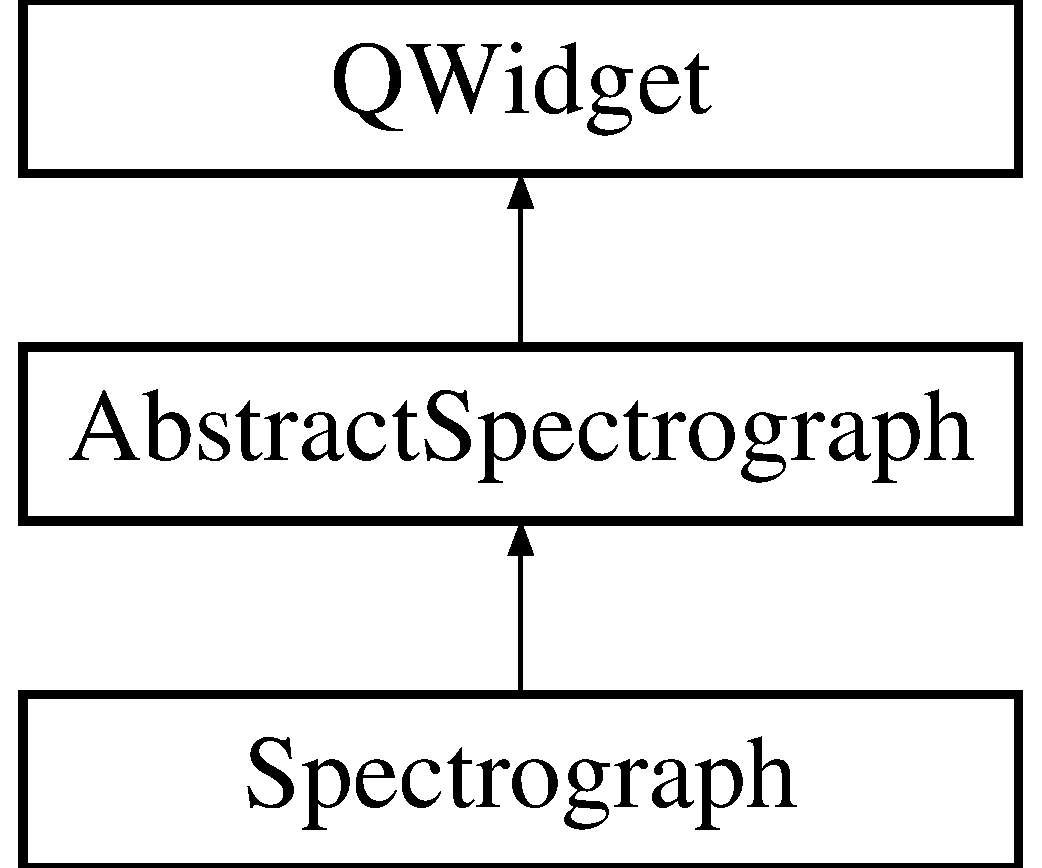
\includegraphics[height=3.000000cm]{class_spectrograph}
\end{center}
\end{figure}
\subsection*{Slots públicos}
\begin{DoxyCompactItemize}
\item 
void \hyperlink{class_spectrograph_a22138fa296829fb5449202f262e64bf5}{paint\-Event} (Q\-Paint\-Event $\ast$e)
\item 
void \hyperlink{class_spectrograph_ae94e6b07459f40c57ed7db97f5d32cf1}{load\-Samples} (Q\-Vector$<$ double $>$ \&\-\_\-spectrum)
\item 
void \hyperlink{class_spectrograph_af690851ad862181732979bdfa88b2dbe}{timer\-Event} (Q\-Timer\-Event $\ast$e)
\item 
void \hyperlink{class_spectrograph_a06514c3f632bc47c7da2cfd66330e85e}{resize\-Event} (Q\-Resize\-Event $\ast$e)
\item 
void \hyperlink{class_spectrograph_aeb2d9200c513b1de462de5f16c4cb0ca}{load\-Levels} (double left, double right)
\end{DoxyCompactItemize}
\subsection*{Membros públicos}
\begin{DoxyCompactItemize}
\item 
\hypertarget{class_spectrograph_ae4a10124a7de6cec48ccd09db0ab5fb6}{{\bfseries Spectrograph} (Q\-Widget $\ast$parent=0)}\label{class_spectrograph_ae4a10124a7de6cec48ccd09db0ab5fb6}

\end{DoxyCompactItemize}


\subsection{Documentação dos métodos}
\hypertarget{class_spectrograph_aeb2d9200c513b1de462de5f16c4cb0ca}{\index{Spectrograph@{Spectrograph}!load\-Levels@{load\-Levels}}
\index{load\-Levels@{load\-Levels}!Spectrograph@{Spectrograph}}
\subsubsection[{load\-Levels}]{\setlength{\rightskip}{0pt plus 5cm}void Spectrograph\-::load\-Levels (
\begin{DoxyParamCaption}
\item[{double}]{left, }
\item[{double}]{right}
\end{DoxyParamCaption}
)\hspace{0.3cm}{\ttfamily [slot]}}}\label{class_spectrograph_aeb2d9200c513b1de462de5f16c4cb0ca}
brief Loads left and right mean audio values \hypertarget{class_spectrograph_ae94e6b07459f40c57ed7db97f5d32cf1}{\index{Spectrograph@{Spectrograph}!load\-Samples@{load\-Samples}}
\index{load\-Samples@{load\-Samples}!Spectrograph@{Spectrograph}}
\subsubsection[{load\-Samples}]{\setlength{\rightskip}{0pt plus 5cm}void Spectrograph\-::load\-Samples (
\begin{DoxyParamCaption}
\item[{Q\-Vector$<$ double $>$ \&}]{\-\_\-spectrum}
\end{DoxyParamCaption}
)\hspace{0.3cm}{\ttfamily [slot]}}}\label{class_spectrograph_ae94e6b07459f40c57ed7db97f5d32cf1}
brief Load samples to be displayed \hypertarget{class_spectrograph_a22138fa296829fb5449202f262e64bf5}{\index{Spectrograph@{Spectrograph}!paint\-Event@{paint\-Event}}
\index{paint\-Event@{paint\-Event}!Spectrograph@{Spectrograph}}
\subsubsection[{paint\-Event}]{\setlength{\rightskip}{0pt plus 5cm}void Spectrograph\-::paint\-Event (
\begin{DoxyParamCaption}
\item[{Q\-Paint\-Event $\ast$}]{e}
\end{DoxyParamCaption}
)\hspace{0.3cm}{\ttfamily [slot]}}}\label{class_spectrograph_a22138fa296829fb5449202f262e64bf5}
brief Paints the screen for spectrum displaing \hypertarget{class_spectrograph_a06514c3f632bc47c7da2cfd66330e85e}{\index{Spectrograph@{Spectrograph}!resize\-Event@{resize\-Event}}
\index{resize\-Event@{resize\-Event}!Spectrograph@{Spectrograph}}
\subsubsection[{resize\-Event}]{\setlength{\rightskip}{0pt plus 5cm}void Spectrograph\-::resize\-Event (
\begin{DoxyParamCaption}
\item[{Q\-Resize\-Event $\ast$}]{e}
\end{DoxyParamCaption}
)\hspace{0.3cm}{\ttfamily [slot]}}}\label{class_spectrograph_a06514c3f632bc47c7da2cfd66330e85e}
brief Redefines some variables when the widget is resized \hypertarget{class_spectrograph_af690851ad862181732979bdfa88b2dbe}{\index{Spectrograph@{Spectrograph}!timer\-Event@{timer\-Event}}
\index{timer\-Event@{timer\-Event}!Spectrograph@{Spectrograph}}
\subsubsection[{timer\-Event}]{\setlength{\rightskip}{0pt plus 5cm}void Spectrograph\-::timer\-Event (
\begin{DoxyParamCaption}
\item[{Q\-Timer\-Event $\ast$}]{e}
\end{DoxyParamCaption}
)\hspace{0.3cm}{\ttfamily [slot]}}}\label{class_spectrograph_af690851ad862181732979bdfa88b2dbe}
brief Used to modify spectrum while a new sample does not arrive 

A documentação para esta classe foi gerada a partir dos seguintes ficheiros\-:\begin{DoxyCompactItemize}
\item 
spectrograph.\-h\item 
spectrograph.\-cpp\end{DoxyCompactItemize}

%--- End generated contents ---

% Index
\newpage
\phantomsection
\addcontentsline{toc}{chapter}{Index}
\printindex

\end{document}
